\section*{\hfil Структура проекта\hfil}

%\noindent\hrulefill
%\begin{figure}[H]
%	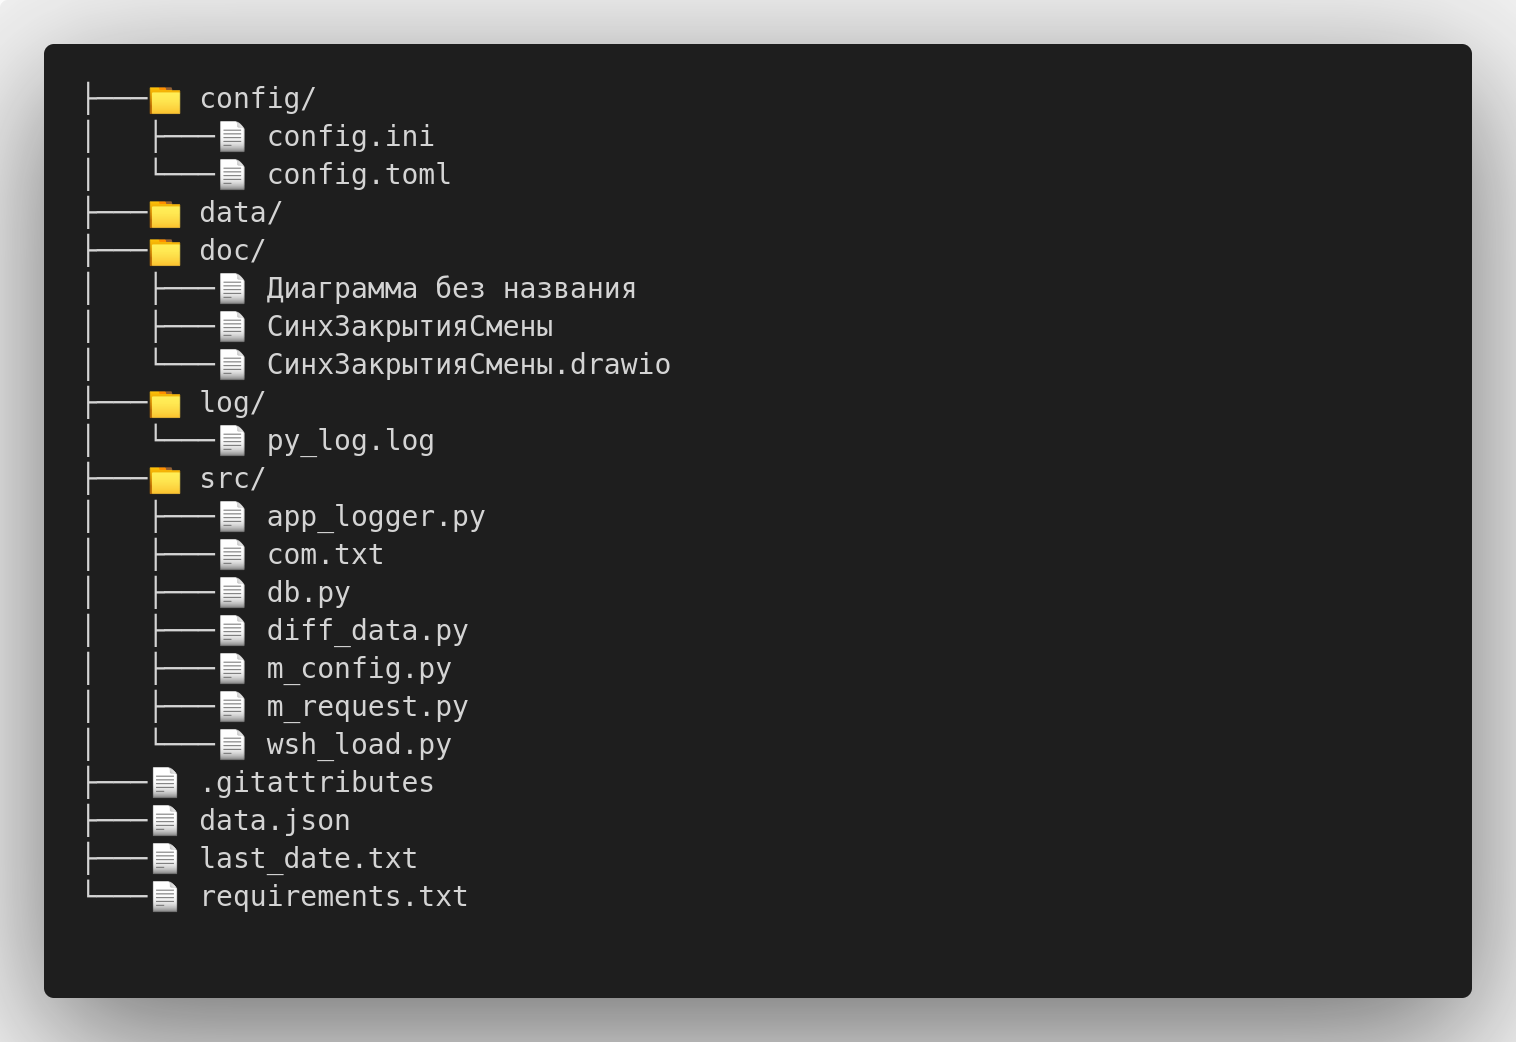
\includegraphics[width=0.95\textwidth]{code.png}
%	\caption{<<Структура проекта>>.}
%	\label{ris:code.png}
%\end{figure}

\renewcommand*\DTstylecomment{\rmfamily\color{blue}\sffamily}
\renewcommand*\DTstyle{\ttfamily\textcolor{black}}
\setlength{\DTbaselineskip}{20pt}
%\DTsetlength{1em}{3em}{0.1em}{1pt}{4pt}

\dirtree{%
	.1 /.	
	.1 Workshift\_load.
	.2 config.\DTcomment{каталог с файлами настроек}.
	.3 config.ini\ldots{} \begin{minipage}[t]{5cm}
		Файл содержит настройки программы{.}
	\end{minipage}.
	.2 log.\DTcomment{каталог с файлами лога}.
	.3 py\_log.log\DTcomment{файл лога}.
	.2 src.\DTcomment{каталог с файлами программы}.
	.3 app\_logger.py.\DTcomment{работа с логированием}.
	.3 db.py.\DTcomment{Работа с БД}.	
	.3 diff\_data.py.\ldots{} \begin{minipage}[t]{5cm}
		Файл содержит тексты запросов{.}
	\end{minipage}.
	.3 m\_config.py.\DTcomment{работа с конфигурацией}.	
	.3 m\_request.py.\DTcomment{работа с Http-запросами}.		
	.3 wsh\_load.py.\DTcomment{основной файл программы}.				
	.3 last\_date\_open.txt.\DTcomment{дата последней открытой смены ККМ}.	
	.3 last\_date.txt.\DTcomment{дата последней закрытой смены ККМ}.	
	.3 first.dat.\ldots{} \begin{minipage}[t]{5cm}
		Файл появляется после первого запуска программы
		если он отсутствует, то при запуске происходит 
		инициализация файлов с датами смен ККМ{.}
	\end{minipage}.
	.1 requirements.txt.\ldots{} \begin{minipage}[t]{5cm}
		Файл содержит наименование и версии установленных 
		модулей подключенных к программе, используется
		при начальной установке{.}
	\end{minipage}.
}
\newpage

\section{Алгоритм}

\begin{itemize}
\item При запуске программы происходит чтение настроек. Если чтение удачно, запускается функция <<main()>>, в противном случае программа завершает свою работу.

%\begin{figure}[H]
%	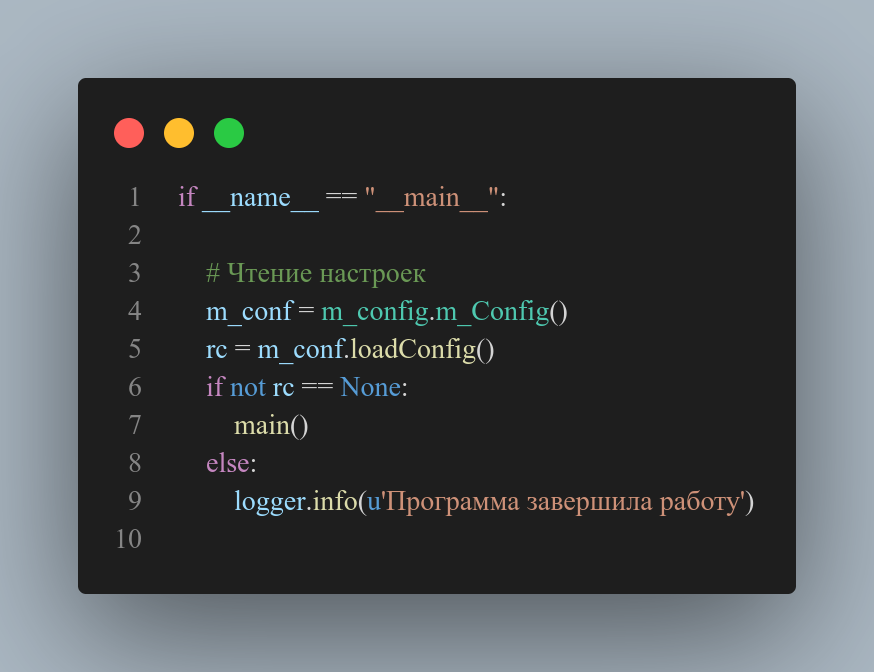
\includegraphics[width=0.65\textwidth]{code1.png}
%	\caption{<<Структура проекта>>.}
%	\label{ris:code1.png}
%\end{figure}


\begin{tcolorbox}
	\begin{lstlisting}[language=Python,ndkeywordstyle=\color{darkgray}\bfseries,identifierstyle=\color{black},stringstyle=\color{red}\ttfamily,showstringspaces=false,keepspaces=true,extendedchars=\true]
if __name__ == "__main__":

	# Чтение настроек
	m_conf = m_config.m_Config()   
	rc =  m_conf.loadConfig()
	if not rc == None:
		main()
	else:
		logger.info(u'Программа завершила работу') 
	\end{lstlisting}
\end{tcolorbox}

\par

\item При запуске функции <<main()>> происходит соединение с базой данных и создается объект для работы с ней, так же создается объект для работы с Http запросами.

\begin{tcolorbox}
	\begin{lstlisting}[language=Python,ndkeywordstyle=\color{darkgray}\bfseries,identifierstyle=\color{black},stringstyle=\color{red}\ttfamily,showstringspaces=false,keepspaces=true,extendedchars=\true]
    tData = db.workDb(rc)
	rec_con = m_request.req1C(rc)
	\end{lstlisting}
\end{tcolorbox}


\item Получаем список смен которые были открыты с последней зафиксированной даты, если появились новые открытые смены, тогда формируем и отправляем Http запрос в 1С. 
Если код возврата был успешным (\textbf{200}), тогда меняем дату в файле, на дату открытия последней смены.

\begin{tcolorbox}
	\begin{lstlisting}[language=Python,ndkeywordstyle=\color{darkgray}\bfseries,identifierstyle=\color{black},stringstyle=\color{red}\ttfamily,showstringspaces=false,keepspaces=true,extendedchars=\true]
 # Список открытых смен от последнего зафиксированного времени
	l_workshift_open = tData.get_last_workshift_open()
	# Если нечего отправлять, то не отправляем
	if len(l_workshift_open) > 0:
		status_code = rec_con.post_workshift_open(l_workshift_open)
	# Меняем дату в файле только в случае успешного результата работы 1C
		if status_code == 200:
			tData.save_new_date_open()
		else:
			logger.info(u'status_code_open - ' + str(status_code ))
	\end{lstlisting}
\end{tcolorbox}


\item Получаем список смен которые были закрыты с последней зафиксированной даты, если появились новые закрытые смены, тогда формируем и отправляем Http запрос в 1С. 
Если код возврата был успешным (\textbf{200}), тогда меняем дату в файле, на дату закрытия последней смены.

\begin{tcolorbox}
	\begin{lstlisting}[language=Python,ndkeywordstyle=\color{darkgray}\bfseries,identifierstyle=\color{black},stringstyle=\color{red}\ttfamily,showstringspaces=false,keepspaces=true,extendedchars=\true]
	# Список закрытых смен от последнего зафиксированного времени
	l_workshift = tData.get_last_workshift()
	# Если нечего отправлять, то и  не отправляем
	if len(l_workshift) > 0:
		status_code = rec_con.post_workshift(l_workshift)
	# Меняем дату в файле только в случае успешного результата работы 1С
		if status_code == 200:
			tData.save_new_date()
		else:
			logger.info(u'status_code - ' + str(status_code ))
	\end{lstlisting}
\end{tcolorbox}

\item Завершаем работу программы.

\end{itemize}